\chapter{Méthodes numériques} \label{chap: methodes_numeriques}

\section{Théorie de champ moyen dynamique sur amas (CDMFT)} \label{sec: cdmft}

La théorie de champ moyen dynamique sur amas~\cite{KOTLIAR}, une extension de la théorie de champ moyen dynamique (DMFT : \textit{Dynamical Mean Field Theory})\footnote{La DMFT~\cite{dmft}, est un cas particulier de la CDMFT où l'amas se réduit à un seul site. La CDMFT est plus sophistiquée car elle capture mieux les corrélations spatiales à courte portée.}est la méthode sur laquelle ce travail est basé. Elle fait partie des méthodes numériques permettant la résolution de modèles d'électrons fortement corrélés. Comme son nom l'indique, le concept d'amas est utilisé comme point de départ de la méthode, exactement comme la CPT~\cite{cpt-david-michel, CptDavid}. Toutefois, contrairement à cette dernière, la CDMFT tient compte de l'effet du réseau sur l'amas choisi via le concept de \textit{bain}. L'idée est de plonger l'amas dans un bain (sans interaction $U$) qui représente la partie du réseau qui est ignorée lorsqu'on se limite à un amas de $N_c$ sites. Les électrons du système peuvent ainsi voyager librement entre les sites de l’amas et du bain. Au fond, il ne s'agit que de degrés de liberté supplémentaires pour les électrons, car, dans un réseau cristallin, il n'y a aucune raison pour ceux-ci d'être confinés à un amas de taille arbitraire. C'est pourquoi l'astuce du bain, pouvant théoriquement accueillir une infinité d'électrons, représente davantage la physique d'un réseau infini. Cette idée est représentée schématiquement sur la figure~\ref{fig: cdmft}.
\begin{figure}[htb!]
    \centering
    \subfloat[]{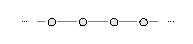
\includegraphics[clip, scale=2.25, trim=0 -0.37cm -0.33cm 0]{figs/methode/cdmft1.pdf}\label{subfig: cdmft1}}
    \subfloat[]{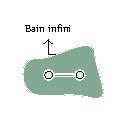
\includegraphics[clip, scale=2.25, trim=0  -0.11cm -0.5cm 0]{figs/methode/cdmft2.pdf}\label{subfig: cdmft2}}
    \subfloat[]{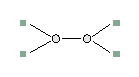
\includegraphics[clip, scale=2.25, trim=0 -0.09cm 0 0.05cm]{figs/methode/cdmft3.pdf}\label{subfig: cdmft3}}
    \caption[Traitement d'un réseau unidimensionnel en CDMFT.]{\textbf{Traitement d'un réseau unidimensionnel en CDMFT.}
    \textbf{(a)} Réseau unidimensionnel infini régit par le modèle de Hubbard.
    \textbf{(b)} Amas de deux sites plongé dans un bain infini sans interaction.
    \textbf{(c)} Discrétisation du bain.}
    \label{fig: cdmft}
\end{figure}
La suite de la méthode CDMFT consiste à résoudre exactement le modèle composé de sites d'amas et d'orbitales de bain. On utilise l'expression «\,orbitales de bain\,», puisque, conceptuellement, ces degrés de liberté n'ont pas de position physique, ce sont des orbitales fictives connectées au périmètre de l'amas. Notons ici que l'on considère un bain discret~\ref{subfig: cdmft3}, car il n'est pas toujours possible de simuler un bain infini~\ref{subfig: cdmft2}. C'est une contrainte associée au solutionneur d'impureté, la diagonalisation exacte, basée sur le formalisme hamiltonien, alors que le Monte-Carlo quantique est quant à lui basé sur le formalisme d'action qui permet la définition d'un bain \textit{continu}. Le but de calculer exactement la fonction de Green amas-bain est d'en extraire la self-énergie $\vb{\Sigma}_c(z)$. On utilise cette self-énergie locale (d'un point de vue de l'amas) avec la relation CPT pour obtenir l'approximation de la fonction de Green réseau.
\begin{figure}[h!]
    \centering
    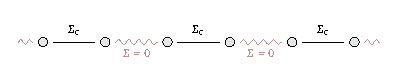
\includegraphics[scale=2.15]{figs/methode/cdmft-self-k.pdf}
    \caption{Approximation de la self-énergie en CDMFT.}
    \label{fig: cdmft-self-k}
\end{figure}
La figure~\ref{fig: cdmft-self-k} met en évidence l'approximation locale de la self-énergie en CDMFT, le principe fondamental qui définit et caractérise cette méthode.
